\documentclass{formation}
\title{Machine Learning}
\subtitle{TP 1 : données et statistiques}

\begin{document}

\maketitle

\begin{frame}
  \frametitle{python}
  Useful tools
  \begin{itemize}
  \item virtualenv
  \item pip
  \item ipython
  \item ipython notebook
  \item \url{conda.pydata.org}
  \end{itemize}
\end{frame}

\begin{frame}
  \frametitle{python}
  Notes
  \begin{itemize}
    \item \texttt{pip install -r requirements.txt}
    \item ipython offers tab completion (vs python)
    \item ipython notebook opens in a browser, caches cell output but not cell state
  \end{itemize}
\end{frame}

\begin{frame}
  \frametitle{pandas}
  \inputminted{python}{pandas_1.py}
\end{frame}

\begin{frame}
  \frametitle{pandas}
  \texttt{Dataframe} has many constructors.  For example,
  \inputminted[linenos,fontsize=\small]{python}{pandas_2.py}
\end{frame}

\begin{frame}
  \frametitle{pandas}
  \purple{Viewing data}
  \inputminted[linenos,fontsize=\small]{python}{pandas_3.py}
\end{frame}

\begin{frame}
  \frametitle{pandas}
  \purple{Basic data exploration}
  \inputminted[linenos,fontsize=\small]{python}{pandas_4.py}
\end{frame}

\begin{frame}
  \frametitle{pandas}
  \purple{Select a column (series)}
  \inputminted[linenos,fontsize=\small]{python}{pandas_5.py}
\end{frame}

\begin{frame}
  \frametitle{pandas}
  \purple{Select a range}
  \inputminted[linenos,fontsize=\small]{python}{pandas_6.py}
\end{frame}

\begin{frame}
  \frametitle{pandas}
  \purple{Boolean selection criteria}
  \inputminted[linenos,fontsize=\small]{python}{pandas_7.py}
\end{frame}

\begin{frame}
  \frametitle{pandas}
    \purple{Recommended}
    \vspace{5mm}
    \url{http://www.gregreda.com/2013/10/26/intro-to-pandas-data-structures/}
\end{frame}

\begin{frame}
  \frametitle{Plotting}
  \begin{minipage}[c]{0.49\linewidth}
    \purple{Draw a line}
    \inputminted[linenos,fontsize=\small]{python}{pyplot_1.py}
  \end{minipage}\hfill
  \begin{minipage}[c]{0.49\linewidth}
    \imgtw[1]{pyplot_1.png}
  \end{minipage}\hfill
\end{frame}

\begin{frame}
  \frametitle{Plotting}
  \begin{minipage}[c]{0.55\linewidth}
    \purple{Draw a line}
    \inputminted[linenos,fontsize=\small]{python}{pyplot_2.py}
  \end{minipage}\hfill
  \begin{minipage}[c]{0.43\linewidth}
    \imgtw[1]{pyplot_2.png}
  \end{minipage}\hfill
\end{frame}

\begin{frame}
  \frametitle{Plotting}
  \purple{Draw a line}
  \inputminted[linenos,fontsize=\small]{python}{pyplot_3.py}
  \vspace{-55mm}
  \flushright{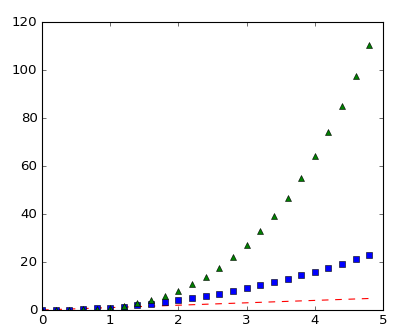
\includegraphics[width=.5\textwidth]{pyplot_3.png}}
\end{frame}

\begin{frame}
  \frametitle{Plotting}
  \purple{Draw two curves}
  \inputminted[linenos,fontsize=\small]{python}{pyplot_4.py}
\end{frame}

\begin{frame}
  \frametitle{Plotting}
  \imgth[0.9]{pyplot_4.png}
\end{frame}

\begin{frame}
  \frametitle{Plotting}
  \purple{Histogram}
  \inputminted[linenos,fontsize=\small]{python}{pyplot_5.py}
\end{frame}

\begin{frame}
  \frametitle{Plotting}
  \imgth[0.9]{pyplot_5.png}
\end{frame}

\begin{frame}
  \frametitle{Plotting}
  \purple{Scatter plot}
  \inputminted[linenos,fontsize=\small]{python}{pyplot_6.py}
\end{frame}

\begin{frame}
  \frametitle{Plotting}
  \imgtw[0.9]{pyplot_6.png}
\end{frame}


\begin{frame}
  \frametitle{Plotting}
    \url{http://matplotlib.org/users/pyplot_tutorial.html}
    \url{http://matplotlib.org/users/beginner.html}
\end{frame}

\end{document}
%%% Local Variables:
%%% mode: latex
%%% TeX-master: t
%%% End:
